% !TeX root = ../main.tex

\begin{figure}[htbp]
  \centering
  
\includegraphics[trim=200 200 200 200, clip, width=0.45\textwidth]{figures/surf-side.png}
  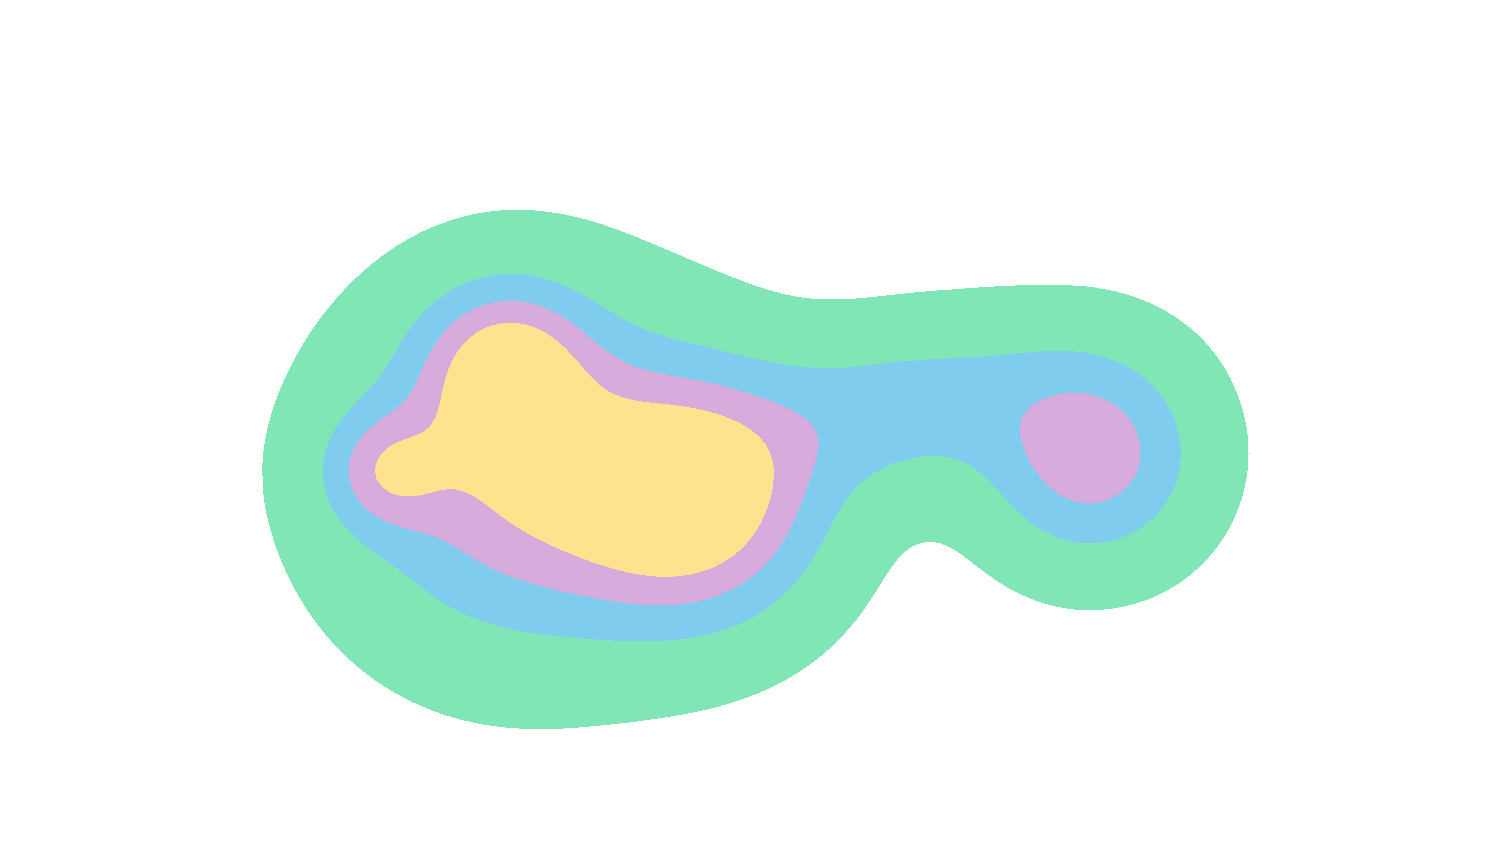
\includegraphics[trim=250 0 50 100, clip, width=0.35\textwidth]{figures/surf-top.png}
  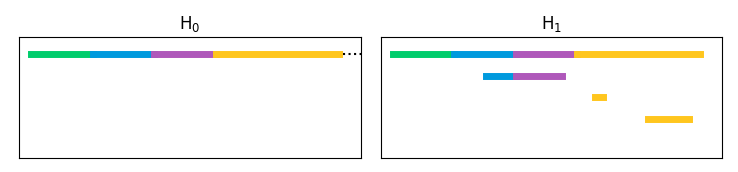
\includegraphics[width=0.8\textwidth]{figures/scalar_barcode_true.png}
  \caption{A scalar field on a 2D domain and its persistence barcode.}
\end{figure}

\paragraph*{Contribution}

We will re-cast the TCC as a way to verify that the persistent homology of a scalar field can be \emph{partially} approximated by a given sample.
Specifically, we will relate the persistent homology of a function relative to a \emph{static} sublevel set to a \emph{truncation} of the full diagram.
That is, beyond a certain point the full diagram remains unchanged, allowing for possible reconstruction.
This is in comparison with the \emph{restricted} diagram obtained by simply ignoring part of the domain.
We therefore present relative persistent homology as an alternative to restriction in a way that extends the TCC to the analysis of scalar fields.

Section~\ref{sec:summary} establishes notation and provides an overview of our main results in Sections~\ref{sec:tcc} and~\ref{sec:middle}.
In Section~\ref{sec:truncations} we introduce an interpretation of the relative diagram as a truncation of the full diagram that is motivated by a number of experiments in Section~\ref{sec:experiments}.
